\DeclareUnicodeCharacter{2028}{} 
\documentclass{article}
\usepackage[dvipsnames]{xcolor}
\usepackage{listings}
\usepackage[section]{placeins}
\usepackage{blindtext}
\usepackage[T1]{fontenc}
\usepackage[utf8]{inputenc}
\usepackage{titling}
\usepackage{float}
\usepackage{tikz}
\usetikzlibrary{calc}
\usetikzlibrary{arrows.meta}
\usepackage{graphicx}
\usepackage[hidelinks]{hyperref}





\title{ Design Document\\2020-2021}
\author{Alessandro Polidori (Codice persona 10573078)\\Olimpia Rivera (Codice persona 10617517)}
\date{}



\renewcommand{\contentsname}{Table of Contents}


\begin{document}

\renewcommand{\labelitemi}{\normalfont -} 

\begin{figure}[]
  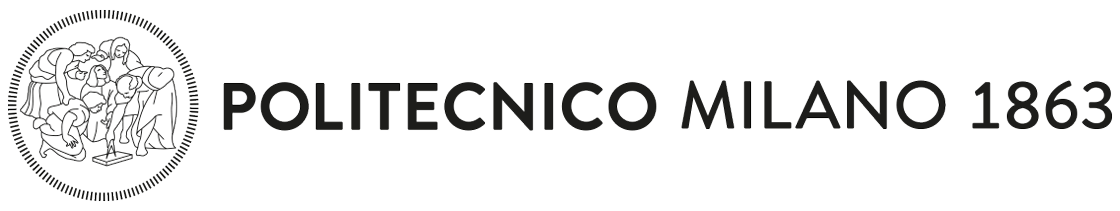
\includegraphics[width=\linewidth]{logo_politecnico copia.png}
  
\end{figure}
\maketitle
\tableofcontents{}
\newpage

\section{Introduction}
\subsection{Purpose}
The purpose of this document is to further detail the software system discussed in the RASD by providing more technical and precise informations. The RASD, indeed, describes the system in terms of requirements, assumptions and goals and gives a general overview of the main system’s functionalities, whereas the DD goes deeper into software design and architecture. In particular, all the required components of the system and the interactions among them are presented, as well as run-time processes and motivated design choices. In addition, the document describes the implementation, integration and testing plans.\\
The relevant issues explored in the Design Document are the following:
\begin{itemize}
\item High-level architecture
\item Main components and relative interfaces
\item Runtime behavior
\item Design patterns
\item Implementation, integration and testing plan
\end{itemize}
This document represents a vehicle for stakeholders communication, as it defines a set of design  decisions made to offer both the essential functionalities and the required quality attributes.

\subsection{Scope}
The CLup software application is designed to help both common users and store managers to deal with some relevant difficulties and challenges created by the coronavirus emergency. The CLup system, indeed, gives users the possibility to join virtual lines to stores and wait for their turn at home instead of standing in line outside stores. The system itself notifies users when it is time to leave to reach the store. Alternatively, thanks to the CLup application, users can choose to book visits to stores in advance, by selecting the preferred date and time slot.
 In order for the lining up mechanism to work effectively, all the users are asked to provide their expected shopping duration and the system will calculate, and eventually modify, the waiting times of the users in line by taking into account the following events: users currently in line, users currently in the store, users getting out of the line, cancelled reservations, crowdedness of stores’ departments and users’ visits’ durations. Indeed, a QR code will be generated for each user and scanned at entrances and exits by smart turnstiles, so that the system can collect and store informations about visits’ duration. The influx of people is managed by the system in an even finer way, by asking users to provide a list of product categories they intend to purchase. The system is also designed to regulate accesses to stores in order to respect restrictions imposed by the virus emergency, by taking into account the stores’ capacities. For this reason, store managers as well benefit from such a software application because they have the possibility to monitor the number of people in they stores updating in real time.\\
A more detailed overview of the functionalities offered by the system can be found in the RASD.

\subsection{Definitions, Acronyms, Abbreviations}
\subsubsection{Definitions}
\subsubsection{Acronyms}
\begin{itemize}
\item RASD: Requirements Analysis and Specifications Document
\item DD: Design Document
\item API: Application Programming Interface
\end{itemize}
\subsubsection{Abbreviations}
\subsection{Revision History}
\subsection{Document Structure}
The Design Document is structured in the following chapters:
\begin{itemize}
\item\textbf{Chapter 1} describes the document’s purpose and scope and its differences with respect to the RASD. Useful specifications (definitions, acronyms, abbreviations) are included for a better understanding of the next sections of the document.
\item\textbf{Chapter 2}
\item\textbf{Chapter 3}
\item\textbf{Chapter 4}
\item\textbf{Chapter 5}
\item\textbf{Chapter 6} presents the effort spent by the group members while working on this project.
\item\textbf{Chapter 7} includes the reference documents.
\end{itemize}

\section{Architectural Design}
\subsection{Overview}
The application architecture is going to be developed as a three-tier architecture. The three logical and physical computing tiers are the following:
\begin{itemize}
\item\textbf{Presentation Tier:} manages the interaction between users and the application. It is responsible for collecting informations form the users and for displaying informations.
\item\textbf{Business logic or Application Tier:} it is where all the communication goes though: it is in charge of processing information collected in the presentation tier and passing it to the data tier. It also manages the way functions are presented to the users.
\item\textbf{Data Access Tier:} it stores and manages the informations processed by the application by performing the necessary operations into the database.
\end{itemize}
More precisely, the architecture is made as a three-tier client-server style, in which presentation, application logic and data processing layers are divided across client and server devices and they all have their own dedicated hardware. The advantages for choosing such an architecture will be further explained in the next sections.
\smallskip\\
Depending on the functionality requested by a user, the client requests a certain service from the server and the invocation of different methods takes place. The server itself provides the needed services through well defined APIs.
\smallskip\\
The functionalities offered by CLup work in the following way:
\begin{itemize}
\item\textbf{Line up:} the application server receives a request of lining up, it takes the required information about the current state of the line from the database server and it sends it back to the client. If the user decides to line up, the application server will communicate with the database server to store the information about the new user, so that the state of the line can be changed. 
\item\textbf{Book visit:} the application server receives a request for booking a visit and provides the user with the necessary forms to complete the reservation. The informations provided by the users will be sent to the application server and then stored in the database.
\item\textbf{Check counter:} the application server will receive the request from the store manager’s client, it takes the information about the counter from the database server and it sends it back to the client.
\item\textbf{Print ticket:} whenever a store manager decides to print a physical ticket, the application server will inform the database server in order for the state of the line to be correctly updated.
\end{itemize}
\subsection{High Level Components}
The following figure represents an high level architecture of the system, showing the different physical machines dedicated to each of the three logic software layers: a tier to interface with the user, a middle tier that holds the business logic of the system, which separates clients and data, and a DataBase Server for the data access layer that holds all the data of the application. \\
\smallskip\\
Not only the modularization of the three layers provides many benefits in terms of flexibility for developers, by allowing them to work on specific part of the application, with minimal impact on the other layers, but it also guarantees more secure accesses to the database. To enhance the overall security of the system, firewalls are installed to monitor and control incoming and outgoing network traffic.
\smallskip\\
Another great advantage of this type of architecture that is exploited is scalability: Application Server and Web Server nodes are replicated and a load-balancing systems are added, improving the overall performance. Note that the Application server and the Web server are considered as a single middle tier containing the business logic, according with the previously defined three-tier architecture. It must be remarked, however, that the Web Server is only used to provide static content (HTML pages).
\smallskip\\
Additionally, reliability and availability are also increased by the usage of a cache on the client side. Indeed, to fasten the process of store selection, the users’ mobile app stores the list of all shops, in order to avoid the connection to the Internet to retrieve the desired one. Consequentially, a mechanism able to keep data up to date is needed.
\smallskip\\
Finally, the clients configuration considered is the Thick one, because it also contains a small part of the business logic. In particular, the clients are able to compute the function that checks whether the waiting time equals the time needed by the user to reach the store. For this reason, the (asynchronous) notification received by the user when it is time to reach the store, is completely managed on the client side.
\smallskip\\
The figure below provides a more detailed, but still very high-level architectural overview, also showing the interaction among the various components.\\
\smallskip\\
As shown in the image, clients’ devices can be either smartphones (for store’s customers), which are connected to the Application Server, or computers (for store’s manager). The Web Servers are used to manage communication with store’s managers’ Web applications: it forwards requests to the Application Server, which ultimately communicates with the Database Server. The Application Server also exploits the Google Maps API in order to retrieve users’ locations.
\subsection{Component view}
\subsection{Deployment View}
In the following deployment diagram the actual physical nodes of the system and the type of used hardware are represented. It also shows the communication methods that occur among the components.\\
\smallskip\\
The nodes show in the image above are the following:
\begin{itemize}
\item\textbf{Smartphone:} together with the store’s computer, it is part of the first tier in which presentation logic must be deployed. The user accesses CLup’s services though this type of device, by communicating with the Application Server, using HTTP. The mobile application must be compatible with the most of the existing Operating Systems, in order to be available on most of the devices.
\item\textbf{Store’s computer:} it is used by store managers (or their employees) to ask for and receive data on the actual crowdedness of their stores. It also sends informations to the Application Server regarding the printing of physical tickets. The communication always takes place through HTTP. The Web Application must be compatible with the most popular Web Browsers.\\
Additionally, on this same node, a piece of software that communicates with the turnstiles is deployed. This communication is fundamental for keeping the customer counter updated. The Application Server, indeed, receives informations about entrances from it, which will eventually be forwarded to the database, in order to keep the state of the store’s crowdedness updated. This piece of software must be able to communicate with the most common turnstiles’ brands.
\item\textbf{Application Server:} it is where most of the application logic is deployed. The mobile application directly forwards all the requests to it, in order to receive the appropriate services. It also handles requests coming from the Web Server, sent by the Web Application.
\item\textbf{Web Server:} it is always part of the middle tier, together with the Application Server. As stated before, however, requests that involve dynamic content (generation of tickets and customer counter), cannot be served by the Web Server. For this reason, these type of requests are forwarded to the Application Server.
\item\textbf{Database Server:}
\end{itemize}
\subsection{Runtime View}
\subsection{Component Interfaces}
\subsection{Selected architectural styles and patterns}
\subsection{Other Design Decisions}
\subsection{Algorithms}

\section{User Interface Design}

\section{Requirements Traceability}

\section{Implementation, Integration and Test Plan}

\section{Effort Spent}

\section{Reference Documents}

\end{document}